\centerline{\Huge \bf  Домашняя работа}
\centerline{\Huge \bf Разрезания. Финал}

\begin{flushright}
    \scriptsize{Только СИГМА сможет решить 4 задачу!}
\end{flushright}

\problem{1!}
Разделите фигуру на четыре равные части. (Разрезать можно не только по линиям клеток, но и по их диагоналям)
\begin{figure}[h]
        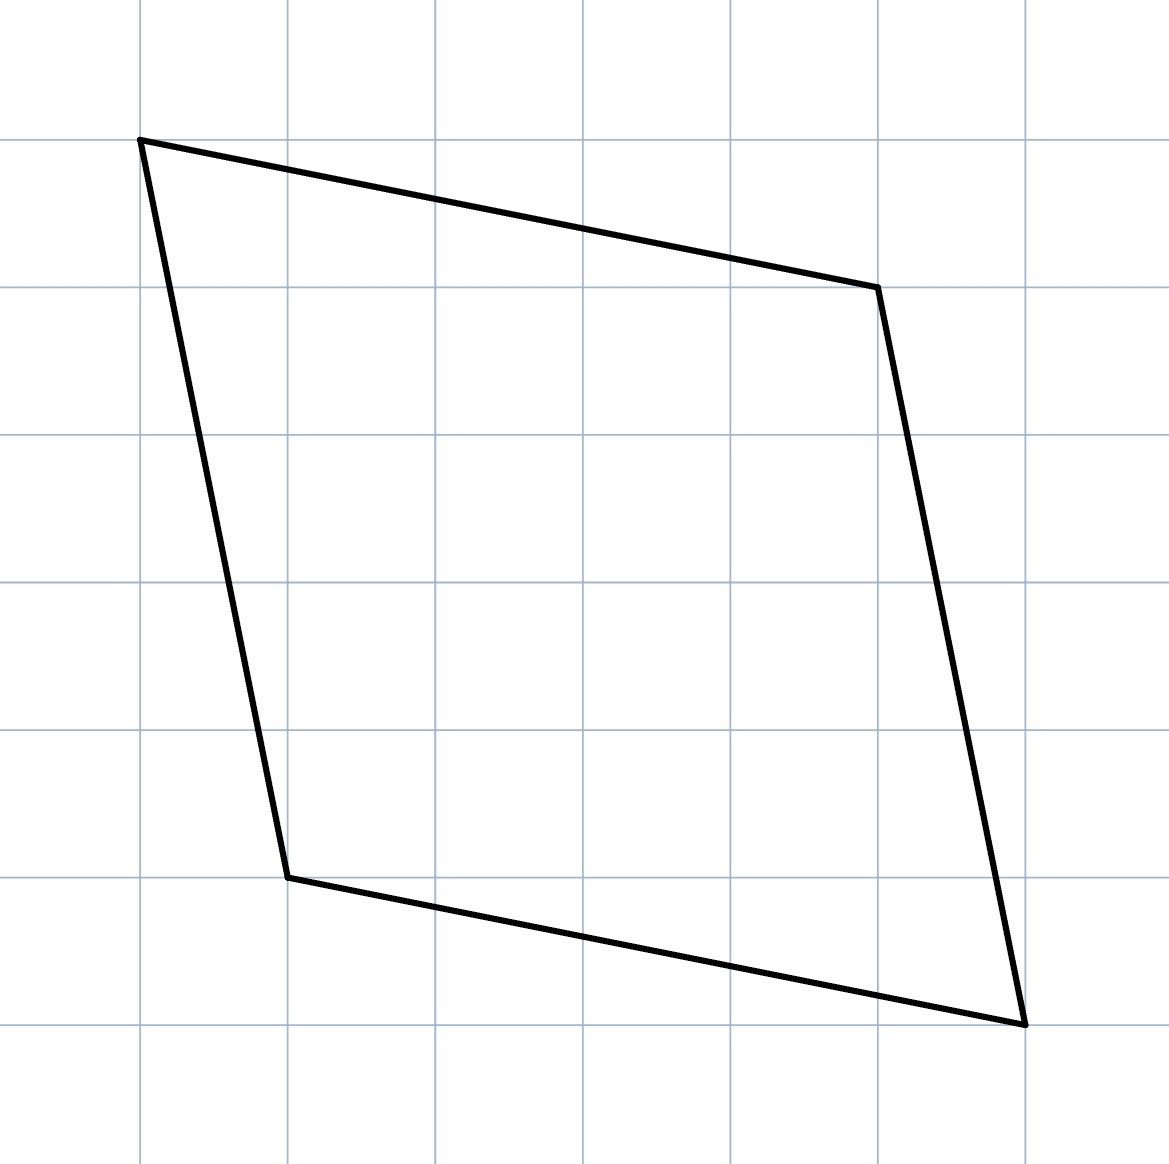
\includegraphics[width=0.2\linewidth]{ЭлМШ 2023-2024/VIII блок/Шиншиллы/HW_Cutting_Final_1.png}
\end{figure}


\problem{2}
Разделите фигуру на три равные части так, чтобы в каждой части была ровно одна точка. (Разрезать можно не только по линиям клеток, но и по их диагоналям)
\begin{figure}[h]
        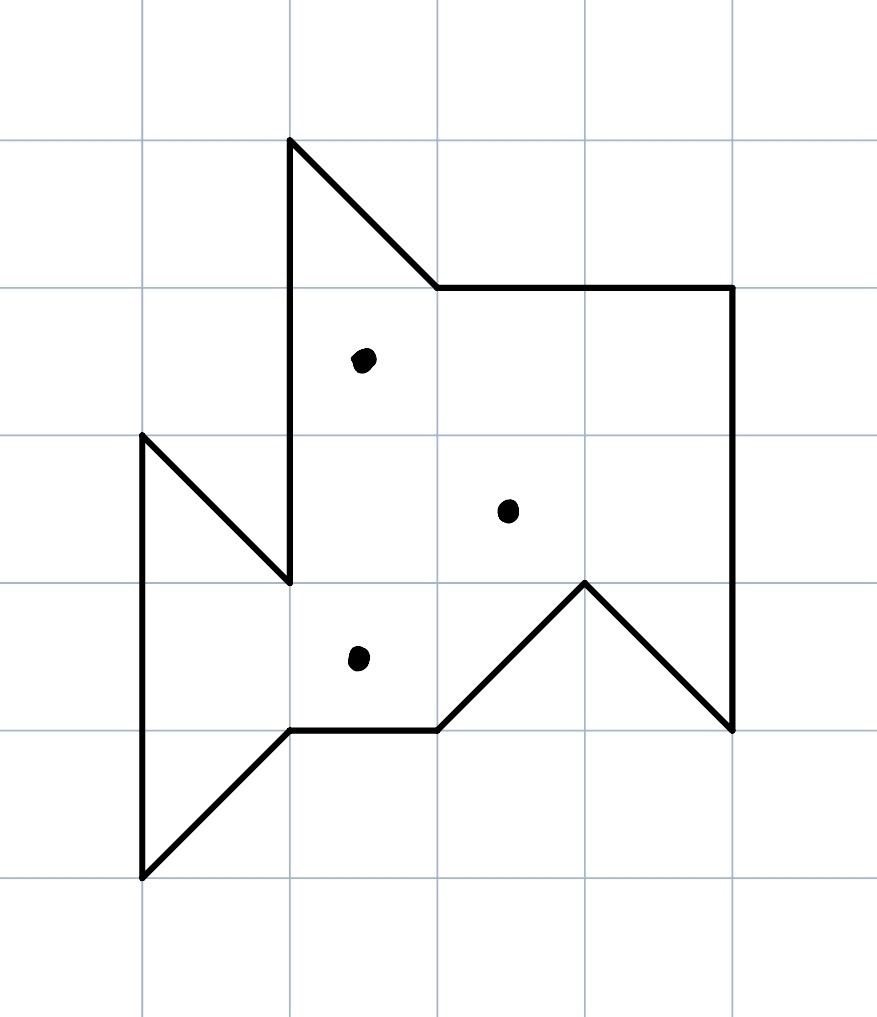
\includegraphics[width=0.2\linewidth]{ЭлМШ 2023-2024/VIII блок/Шиншиллы/HW_Cutting_Final_2.png}
\end{figure}

\problem{3}
Разделите фигуру на восемь равных частей. (Разрезать можно не только по линиям клеток, но и по их диагоналям)
\begin{figure}[h]
        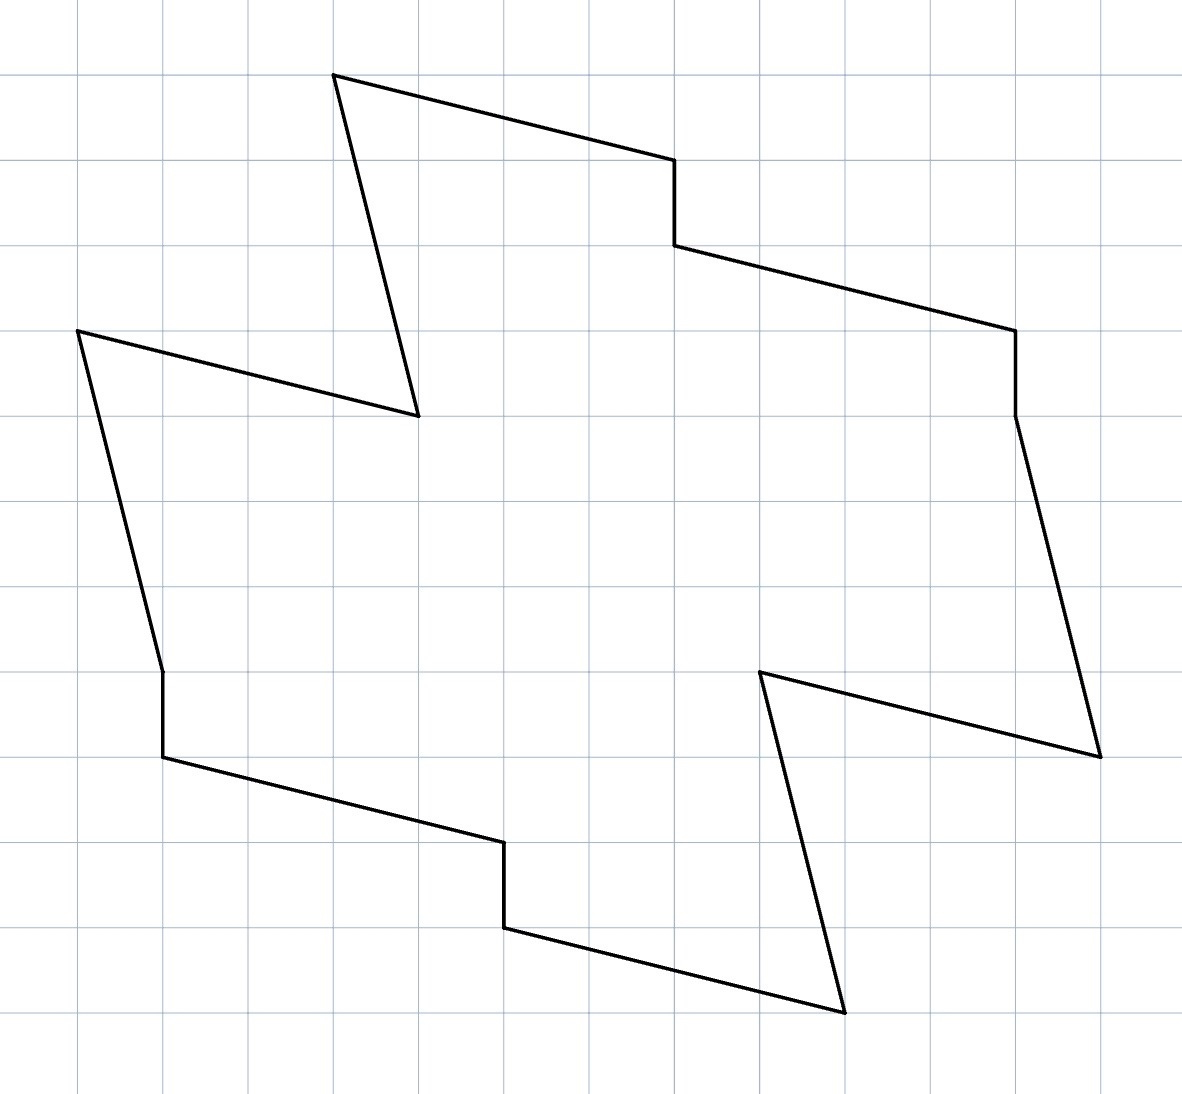
\includegraphics[width=0.2\linewidth]{ЭлМШ 2023-2024/VIII блок/Шиншиллы/HW_Cutting_Final_3.png}
\end{figure}


\newpage

\hspace{3mm}

\problem{4}
\textbf{(Ковёр-СИГМАлёт)} Разделите фигуру на 32 равные части.(Разрезать можно не только по линиям клеток, но и по их диагоналям. Черным закрашены пустоты в фигуре)
\begin{figure}[h]
        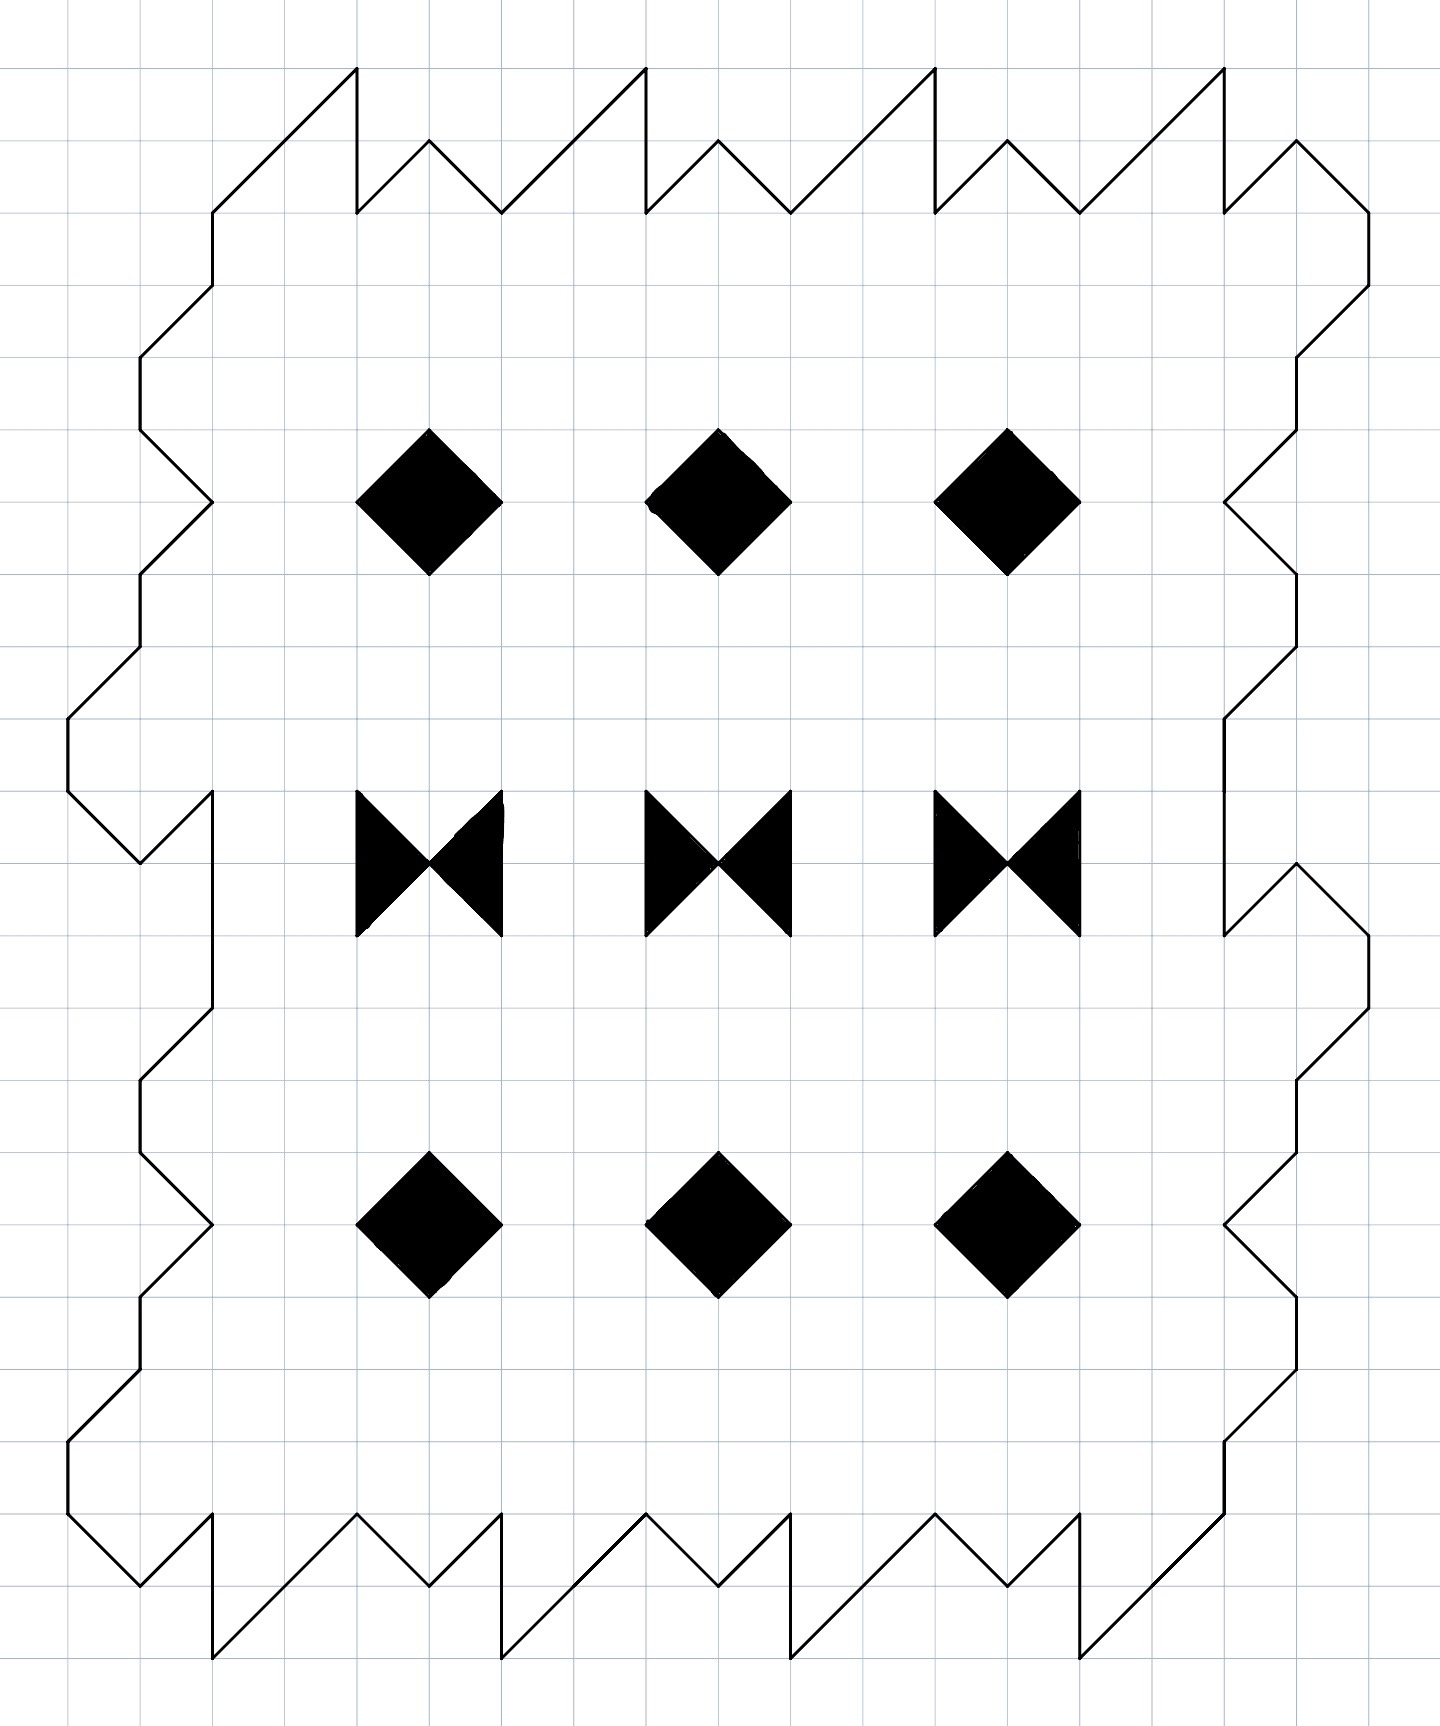
\includegraphics[width=0.2\linewidth]{ЭлМШ 2023-2024/VIII блок/Шиншиллы/HW_Cutting_Final_4.png}
\end{figure}

